% Fig. 1: study design and analysis workflow (five panels, a-e).
% Palette: tints of Paul Tol's "light" qualitative scheme (colour-blind safe), one hue per role:
% yellow = clinical/no image, cyan = foundation-model image block, mint = clinical + image,
% orange = test data, purple = external cohort; indigo accent for structure.
% The three CT slices (LUNG1-001, through the GTV centroid, lung window) are produced by
% scripts/build_figure1_slices.py.
% Build: ../../../.venv/bin/python ../../scripts/build_figure1_slices.py; pdflatex study_overview_fig.tex;
%        cp study_overview_fig.pdf ../study_overview.pdf
\documentclass[tikz,border=1pt]{standalone}
\usepackage[T1]{fontenc}
\usepackage{helvet}
\renewcommand{\familydefault}{\sfdefault}
\renewcommand{\mddefault}{c}
\renewcommand{\bfdefault}{bc}
\usepackage{graphicx}
\usepackage{fix-cm}
\usepackage{amsmath}
\usetikzlibrary{arrows.meta,calc,decorations.pathreplacing}

\definecolor{ink}{HTML}{263040}
\definecolor{muted}{HTML}{6B7686}
\definecolor{accent}{HTML}{34508A}
\definecolor{clinF}{HTML}{FBF1D2}\definecolor{clinE}{HTML}{B8932E}
\definecolor{imgF}{HTML}{DCEFF8}\definecolor{imgE}{HTML}{3F8FB8}
\definecolor{combF}{HTML}{DDF0E7}\definecolor{combE}{HTML}{3A9A72}
\definecolor{testF}{HTML}{F8D9CF}\definecolor{testE}{HTML}{C8603F}
\definecolor{extF}{HTML}{EBDDF0}\definecolor{extE}{HTML}{8A5A9E}
\definecolor{devF}{HTML}{E4E9F3}

\newcommand{\fs}{\fontsize{6.9}{7.7}\selectfont}
\newcommand{\fsm}{\fontsize{6.2}{6.9}\selectfont}

\tikzset{
  >={Latex[length=3.6pt,width=3.2pt]},
  box/.style={rounded corners=1.2pt, line width=0.6pt, align=center, font=\fs, text=ink, inner sep=1.5pt},
  clin/.style={box, fill=clinF, draw=clinE}, img/.style={box, fill=imgF, draw=imgE},
  comb/.style={box, fill=combF, draw=combE}, ext/.style={box, fill=extF, draw=extE},
  plain/.style={box, fill=white, draw=accent!70},
  pill/.style={rounded corners=1.6mm, line width=0.6pt, font=\fs, text=ink, inner xsep=3pt, inner ysep=0pt,
              text height=5.1pt, text depth=0pt},% cap height of the 6.9-7.3pt font, so capitals sit centred
  tile/.style={rounded corners=1.5pt, fill=devF, draw=accent!45, line width=0.45pt},
  title/.style={font=\fontsize{7.9}{8.8}\selectfont\bfseries, text=accent, align=left, anchor=north west},
  badge/.style={circle, fill=accent, text=white, inner sep=0, minimum size=0.36cm,
                font=\fontsize{8}{8}\selectfont\bfseries},
  flow/.style={->, line width=0.65pt, draw=ink},
  thin/.style={line width=0.5pt, draw=ink},
  lab/.style={font=\fsm, text=ink, align=center},
}

% Icons ---------------------------------------------------------------
\newcommand{\snowflake}[2][1]{% frozen weights
  \begin{scope}[shift={#2}, scale=#1]
    \foreach \a in {90,150,...,450} {
      \draw[line width=0.5pt, draw=imgE, line cap=round] (0,0) -- (\a:0.13);
      \draw[line width=0.4pt, draw=imgE, line cap=round] (\a:0.08) -- ++(\a+40:0.04) (\a:0.08) -- ++(\a-40:0.04);}
  \end{scope}}
\newcommand{\funnel}[1]{% quality filter
  \begin{scope}[shift={#1}]
    \draw[thin, fill=white, line join=round] (-0.17,0.17) -- (0.17,0.17) -- (0.04,0.0) -- (0.04,-0.16) -- (-0.04,-0.11) -- (-0.04,0.0) -- cycle;
    \foreach \p in {(-0.07,0.25),(0.02,0.29),(0.09,0.24)} \fill[clinE] \p circle (0.025);
  \end{scope}}
\newcommand{\kmcurve}[1]{% survival curve in a small frame centred at #1
  \begin{scope}[shift={#1}]
    \draw[line width=0.5pt, draw=accent!60, fill=white, rounded corners=1pt] (-0.25,-0.22) rectangle (0.25,0.22);
    \draw[thin, line width=0.35pt] (-0.18,0.15) -- (-0.18,-0.15) -- (0.19,-0.15);
    \draw[line width=0.6pt, draw=accent] (-0.18,0.12) -| (-0.1,0.06) -| (-0.02,-0.01) -| (0.05,-0.05) -| (0.12,-0.09) -- (0.18,-0.09);
  \end{scope}}
\newcommand{\chevron}[1]{% arrow between panels
  \fill[accent!80] ($#1+(-0.11,0.17)$) -- ++(0.1,0) -- ++(0.13,-0.17) -- ++(-0.13,-0.17) -- ++(-0.1,0) -- ++(0.13,0.17) -- cycle;}
\newcommand{\person}[1]{% patient
  \begin{scope}[shift={#1}]
    \fill[accent!70] (0,0.075) circle (0.05);
    \fill[accent!70] (-0.085,-0.1) -- (-0.085,-0.04) arc (180:0:0.085 and 0.07) -- (0.085,-0.1) -- cycle;
  \end{scope}}

\begin{document}
\begin{tikzpicture}[x=1cm, y=1cm]
\useasboundingbox (0,0.55) rectangle (18.5,7.45);
\def\pa{1.65}\def\pb{5.45}\def\pc{9.25}\def\pd{13.05}\def\pe{16.85}
\foreach \x in {3.55,7.35,11.15,14.95} \chevron{(\x,4.1)};
\foreach \x/\l/\t in {\pa/a/{Cohorts and\\imaging}, \pb/b/{Foundation model\\representation},
                     \pc/c/{Prespecified\\models}, \pd/d/{Nested\\cross-validation}, \pe/e/{Paired out-of-fold\\evaluation}} {
  \node[badge] at (\x-1.36,7.19) {\l};
  \node[title] at (\x-1.1,7.4) {\t};
  \draw[accent!35, line width=0.6pt] (\x-1.5,6.56) -- (\x+1.5,6.56);
}

% ===================================================== a: cohorts and imaging
\begin{scope}[shift={(\pa,0)}]
\node[plain, minimum width=2.9cm, minimum height=0.66cm] at (0,6.0) {\textbf{Development: LUNG1}\\NSCLC-Radiomics, 422 patients};
\fill[black, rounded corners=2pt] (-1.5,3.82) rectangle (1.5,4.86);
\node[inner sep=0] at (0,4.34) {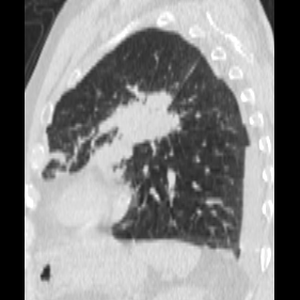
\includegraphics[width=0.92cm]{slice_sagittal_square.png}\hspace{0.5mm}%
  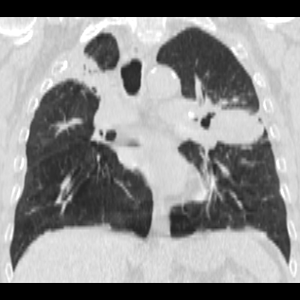
\includegraphics[width=0.92cm]{slice_coronal_square.png}\hspace{0.5mm}%
  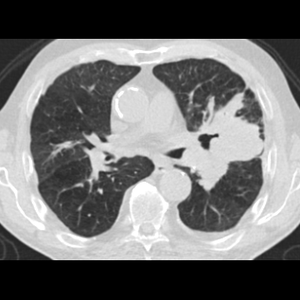
\includegraphics[width=0.92cm]{slice_axial_square.png}};
\draw[flow] (0,5.64) -- (0,5.3);
\node[lab, text=muted] at (0,5.06) {Pretreatment CT, whole volume};
\draw[flow] (0,3.78) -- (0,3.45);
\node[clin, minimum width=2.9cm, minimum height=0.9cm] at (0,2.95) {};
\funnel{(-0.95,2.93)}
\node[font=\fs, text=ink, align=left, anchor=west] at (-0.62,2.95) {\textbf{CT audit}\\416 patients\\369 deaths};
\node[ext, minimum width=2.9cm, minimum height=0.9cm] at (0,1.5) {\textbf{External cohort}\\NSCLC-Radiogenomics\\143 patients};
\end{scope}

% ===================================================== b: foundation models
\begin{scope}[shift={(\pb,0)}]
\foreach \name/\i in {COLIPRI/0, TANGERINE/1, Rad-JEPA-3D/2, CT-CLIP/3, DINOv3 (2D)/4}
  \node[pill, fill=imgF, draw=imgE, minimum width=2.6cm, minimum height=0.33cm,
        font=\fontsize{7.1}{7.8}\selectfont\bfseries] at (0,6.2-\i*0.39) {\name};
% CT volume -> encoder -> embedding
\begin{scope}[shift={(-1.05,3.95)}]
  \draw[thin, fill=white] (-0.22,-0.22) rectangle (0.14,0.14);
  \draw[thin, fill=devF] (-0.22,0.14) -- (-0.14,0.22) -- (0.22,0.22) -- (0.14,0.14) -- cycle;
  \draw[thin, fill=devF!70!ink] (0.14,0.14) -- (0.22,0.22) -- (0.22,-0.14) -- (0.14,-0.22) -- cycle;
\end{scope}
\draw[flow] (-0.78,3.95) -- (-0.55,3.95);
\draw[line width=0.6pt, draw=imgE, fill=imgF, rounded corners=1pt] (-0.5,3.57) -- (0.45,3.75) -- (0.45,4.15) -- (-0.5,4.33) -- cycle;
\snowflake{(-0.03,3.95)}
\draw[flow] (0.5,3.95) -- (0.73,3.95);
\foreach \h [count=\k from 0] in {0.32,0.18,0.42,0.12,0.26,0.36}
  \fill[imgE!70] (0.8+\k*0.1,3.7) rectangle ++(0.07,\h);
\node[lab, text=muted] at (-1.05,3.5) {CT};
\node[lab, text=muted] at (-0.03,3.38) {encoder};
\node[lab, text=muted] at (1.07,3.53) {vector};
\draw[flow, rounded corners=2pt] (1.07,3.42) |- (0.3,3.17) -| (0,2.97);
\node[img, minimum width=2.6cm, minimum height=0.6cm] at (0,2.65) {Global embedding\\whole CT, without GTV};
\draw[box, dashed, draw=imgE, fill=white] (-1.4,1.25) rectangle (1.4,1.85);
\snowflake[1.15]{(-1.07,1.55)}
\node[font=\fs, text=ink, align=left, anchor=west] at (-0.82,1.55) {Frozen encoders\\(adapted only in RQ2)};
\end{scope}

% ===================================================== c: prespecified models
\begin{scope}[shift={(\pc,0)}]
\node[pill, fill=accent, draw=accent, text=white, minimum width=2.75cm, minimum height=0.36cm] at (0,6.22) {\textbf{L2-penalized Cox model}};
\draw[accent, line width=0.6pt] (0,6.04) -- (0,5.92) (-0.78,5.78) |- (0.78,5.92) -- (0.78,5.78);
\foreach \t/\x/\y/\s in {{Clinical}/-0.78/5.45/clin, {Stage +\\Volume}/0.78/5.45/clin,
                        {Clinical +\\Volume}/-0.78/4.7/clin, {Image\\alone}/0.78/4.7/img,
                        {+ Radiomics}/-0.78/3.95/clin, {+ Image}/0.78/3.95/comb,
                        {+ Radiomics\\+ Image}/-0.78/3.2/comb, {Tumour-\\centred}/0.78/3.2/clin}
  \node[\s, minimum width=1.45cm, minimum height=0.62cm] at (\x,\y) {\t};
\foreach \s/\t/\y in {clin/{no foundation model}/2.38, img/{foundation model}/2.08, comb/{clinical + foundation model}/1.78}
  { \draw[\s] (-1.3,\y-0.08) rectangle ++(0.24,0.16); \node[lab, anchor=west] at (-0.98,\y) {\t}; }
\node[lab, text=muted, align=left, anchor=west] at (-1.45,1.2) {+ block: added to Clinical + Volume\\Image: PCA16 of one encoder};
\end{scope}

% ===================================================== d: nested cross-validation
\begin{scope}[shift={(\pd,0)}]
\foreach \i in {0,...,6} \person{(-1.02+\i*0.29,6.22)};
\node[font=\fs\bfseries, text=accent] at (1.05,6.2) {$\cdots$};
\node[lab] at (0,5.9) {416 patients, split once by patient ID};
\draw[flow] (0,5.79) -- (0,5.6);
\node[font=\fs, text=ink] at (0,5.46) {5 outer folds, each tested once};
\foreach \i/\f/\e in {0/devF/accent!60,1/devF/accent!60,2/devF/accent!60,3/devF/accent!60,4/testF/testE}
  \draw[line width=0.5pt, fill=\f, draw=\e] (-1.4+\i*0.56,4.98) rectangle ++(0.56,0.3);
\node[font=\fsm, text=testE!80!black] at (1.12,5.13) {test};
\draw[thin, decorate, decoration={brace, mirror, amplitude=3pt}] (-1.38,4.92) -- (0.8,4.92)
  node[midway, below=2.5pt, lab] (dev) {development (80\%)};
% the development set of each outer fold is split again
\draw[flow] (dev.south) -- (dev.south |- 0,4.18);
\draw[box, fill=white, draw=accent!60] (-1.4,2.3) rectangle (1.4,4.18);
\node[font=\fs, text=ink] at (0,3.97) {3 inner folds};
\node[lab, text=muted] at (0,3.72) {within each development set};
\foreach \i/\f/\e in {0/devF/accent!60,1/devF/accent!60,2/testF!55/testE}
  \draw[line width=0.5pt, fill=\f, draw=\e] (-1.05+\i*0.7,3.17) rectangle ++(0.7,0.3);
\node[lab] at (-0.35,3.03) [anchor=north] {training};
\node[lab] at (0.7,3.03) [anchor=north] {validation};
\node[font=\fs, text=ink] at (0,2.5) {penalty selection};
\draw[combE, line width=0.7pt, line cap=round, line join=round] (-1.25,1.55) -- (-1.15,1.45) -- (-0.98,1.67);
\node[font=\fs, text=ink, align=left, anchor=west] at (-0.85,1.55) {Same folds for every\\model and analysis};
\end{scope}

% ===================================================== e: paired evaluation
\begin{scope}[shift={(\pe,0)}]
\node[lab, text=muted] at (-0.6,6.3) {out-of-fold predictions};
\node[clin, minimum width=1.4cm, minimum height=0.6cm] (ref) at (-0.82,5.8) {Clinical +\\Volume};
\node[comb, minimum width=1.4cm, minimum height=0.6cm] (aug) at (-0.82,4.98) {+ Image\\(e.g.\ COLIPRI)};
\draw[flow] (ref.east) -- (0.06,5.8); \kmcurve{(0.33,5.8)};
\draw[flow] (aug.east) -- (0.06,4.98); \kmcurve{(0.33,4.98)};
\draw[thin, line width=0.55pt] (0.62,5.8) -| (0.74,4.98) -- (0.62,4.98) (0.74,5.39) -- (0.84,5.39);
\node[pill, fill=accent, draw=accent, text=white, minimum width=0.62cm, minimum height=0.36cm,
      font=\fontsize{7.3}{8}\selectfont\bfseries] (dc) at (1.17,5.39) {$\boldsymbol{\mathsf{\Delta}}$C};
\node[lab, anchor=north, align=center] at (1.17,5.15) {same\\patients};
\foreach \y in {3.8,3.22,2.64,2.06}
  \draw[accent!35, line width=0.45pt, dotted] (-1.5,\y) -- (1.5,\y);
\begin{scope}[font=\fs, text=ink]
  \node[anchor=west] at (-0.95,4.09) {Uno's C at 36 months};
  \node[anchor=west] at (-0.95,3.51) {Paired bootstrap 95\% CI};
  \node[anchor=west] at (-0.95,2.93) {Holm correction};
  \node[anchor=west] at (-0.95,2.35) {Equivalence margin \textpm 0.03};
  \node[anchor=west, align=left] at (-0.95,1.55) {External test (RQ4):\\models frozen, used once};
\end{scope}
% row icons on light tiles, centred at x = -1.27
\foreach \y in {4.09,3.51,2.93,2.35} \draw[tile] (-1.44,\y-0.17) rectangle ++(0.34,0.34);
\draw[tile, fill=extF, draw=extE!60] (-1.44,1.38) rectangle ++(0.34,0.34);
% Uno's C at 36 months
\node[text=accent, font=\fontsize{6.8}{7}\selectfont\bfseries, inner sep=0] at (-1.27,4.09) {C\textsubscript{\kern-0.5pt36}};
% bootstrap distribution with its interval
\foreach \k/\h in {0/0.05,1/0.12,2/0.17,3/0.11,4/0.05} \fill[accent!75] (-1.375+\k*0.045,3.44) rectangle ++(0.035,\h);
\draw[accent, line width=0.5pt] (-1.38,3.39) -- (-1.16,3.39) (-1.38,3.36) -- (-1.38,3.42) (-1.16,3.36) -- (-1.16,3.42);
% Holm: ordered p values against a stepped threshold
\foreach \k/\h in {0/0.05,1/0.09,2/0.15,3/0.21} \fill[accent!75] (-1.38+\k*0.055,2.82) rectangle ++(0.04,\h);
\draw[testE, line width=0.5pt] (-1.4,2.89) -- (-1.34,2.89) -- (-1.34,2.93) -- (-1.28,2.93) -- (-1.28,2.97) -- (-1.14,2.97);
% equivalence: interval inside the margin
\fill[combF] (-1.37,2.23) rectangle (-1.17,2.47);
\draw[combE, line width=0.45pt, dashed] (-1.37,2.23) -- (-1.37,2.47) (-1.17,2.23) -- (-1.17,2.47);
\draw[accent, line width=0.55pt] (-1.33,2.35) -- (-1.21,2.35) (-1.33,2.32) -- (-1.33,2.38) (-1.21,2.32) -- (-1.21,2.38);
\fill[accent] (-1.27,2.35) circle (0.028);
% external cohort: globe
\draw[extE, line width=0.5pt] (-1.27,1.55) circle (0.11) (-1.38,1.55) -- (-1.16,1.55) (-1.27,1.55) ellipse (0.05 and 0.11);
\end{scope}

\end{tikzpicture}
\end{document}
